%(BEGIN_QUESTION)
% Copyright 2011, Tony R. Kuphaldt, released under the Creative Commons Attribution License (v 1.0)
% This means you may do almost anything with this work of mine, so long as you give me proper credit

Dette nivåreguleringssystemet ser ikke ut til å regulere væskenivået i tanken korrekt. SP er satt til 2.5 fot (innenfor området 0--5 fot), men PV-visningen på regulatorens front viser 3.74 fot. Du legger også merke til at regulatorutgangen står på 100\%.

$$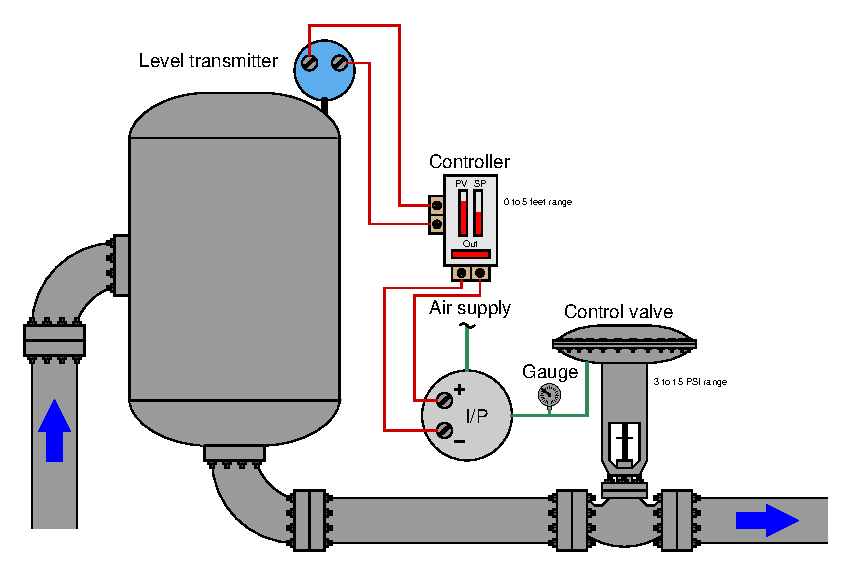
\includegraphics[width=15.5cm]{i00345x01.eps}$$

Første test er å måle sløyfestrøm i kretsen mellom nivåtransmitter og nivåregulator. Multimeteret viser 15.93 mA. Neste steg er å lese av trykkmåleren: 14.99 PSI.

\vskip 10pt

Vurder sannsynligheten for hver oppgitt feil i dette reguleringssystemet. Se på én feil om gangen (altså ingen sammenfallende feil), og avgjør om hver feil alene kan forklare \textit{alle} målinger og symptomer i kretsen.

% No blank lines allowed between lines of an \halign structure!
% I use comments (%) instead, so that TeX doesn't choke.

$$\vbox{\offinterlineskip
\halign{\strut
\vrule \quad\hfil # \ \hfil & 
\vrule \quad\hfil # \ \hfil & 
\vrule \quad\hfil # \ \hfil \vrule \cr
\noalign{\hrule}
%
% First row
{\bf Feil} & {\bf Mulig} & {\bf Umulig} \cr
%
\noalign{\hrule}
%
% Another row
LT ute av kalibrering (sender feil strøm) &  &  \cr
%
\noalign{\hrule}
%
% Another row
LIC-inngang ute av kalibrering (tolker signal feil) &  &  \cr
%
\noalign{\hrule}
%
% Another row
LIC-utgang ute av kalibrering (sender feil mA-signal til I/P) &  &  \cr
%
\noalign{\hrule}
%
% Another row
Trykkmåler ute av kalibrering (viser feil trykk) &  &  \cr
%
\noalign{\hrule}
%
% Another row
I/P ute av kalibrering (gir feil trykk ut) &  &  \cr
%
\noalign{\hrule}
%
% Another row
Reguleringsventilen er overdimensjonert &  &  \cr
%
\noalign{\hrule}
%
% Another row
Reguleringsventilen er underdimensjonert &  &  \cr
%
\noalign{\hrule}
%
% Another row
Ventilens bench-set er feiljustert &  &  \cr
%
\noalign{\hrule}
%
% Another row
LIC er dårlig trimmet &  &  \cr
%
\noalign{\hrule}
%
% Another row
Instrumentluftforsyningen har ikke fullt trykk &  &  \cr
%
\noalign{\hrule}
} % End of \halign 
}$$ % End of \vbox

\underbar{file i00345}
%(END_QUESTION)





%(BEGIN_ANSWER)

% No blank lines allowed between lines of an \halign structure!
% I use comments (%) instead, so that TeX doesn't choke.

$$\vbox{\offinterlineskip
\halign{\strut
\vrule \quad\hfil # \ \hfil & 
\vrule \quad\hfil # \ \hfil & 
\vrule \quad\hfil # \ \hfil \vrule \cr
\noalign{\hrule}
%
% First row
{\bf Feil} & {\bf Mulig} & {\bf Umulig} \cr
%
\noalign{\hrule}
%
% Another row
LT ute av kalibrering (sender feil strøm) & $\surd$ &  \cr
%
\noalign{\hrule}
%
% Another row
LIC-inngang ute av kalibrering (tolker signal feil) &  & $\surd$ \cr
%
\noalign{\hrule}
%
% Another row
LIC-utgang ute av kalibrering (sender feil mA-signal til I/P) &  & $\surd$ \cr
%
\noalign{\hrule}
%
% Another row
Trykkmåler ute av kalibrering (viser feil trykk) &  & $\surd$ \cr
%
\noalign{\hrule}
%
% Another row
I/P ute av kalibrering (gir feil trykk ut) &  & $\surd$ \cr
%
\noalign{\hrule}
%
% Another row
Reguleringsventilen er overdimensjonert &  & $\surd$ \cr
%
\noalign{\hrule}
%
% Another row
Reguleringsventilen er underdimensjonert & $\surd$ &  \cr
%
\noalign{\hrule}
%
% Another row
Ventilens bench-set er feiljustert & $\surd$ &  \cr
%
\noalign{\hrule}
%
% Another row
LIC er dårlig trimmet &  & $\surd$ \cr
%
\noalign{\hrule}
%
% Another row
Instrumentluftforsyningen har ikke fullt trykk &  & $\surd$ \cr
%
\noalign{\hrule}
} % End of \halign 
}$$ % End of \vbox

%(END_ANSWER)





%(BEGIN_NOTES)



%(END_NOTES)
